\documentclass[]{article}\usepackage[]{graphicx}\usepackage[]{color}
%% maxwidth is the original width if it is less than linewidth
%% otherwise use linewidth (to make sure the graphics do not exceed the margin)
\makeatletter
\def\maxwidth{ %
  \ifdim\Gin@nat@width>\linewidth
    \linewidth
  \else
    \Gin@nat@width
  \fi
}
\makeatother

\definecolor{fgcolor}{rgb}{0.345, 0.345, 0.345}
\newcommand{\hlnum}[1]{\textcolor[rgb]{0.686,0.059,0.569}{#1}}%
\newcommand{\hlstr}[1]{\textcolor[rgb]{0.192,0.494,0.8}{#1}}%
\newcommand{\hlcom}[1]{\textcolor[rgb]{0.678,0.584,0.686}{\textit{#1}}}%
\newcommand{\hlopt}[1]{\textcolor[rgb]{0,0,0}{#1}}%
\newcommand{\hlstd}[1]{\textcolor[rgb]{0.345,0.345,0.345}{#1}}%
\newcommand{\hlkwa}[1]{\textcolor[rgb]{0.161,0.373,0.58}{\textbf{#1}}}%
\newcommand{\hlkwb}[1]{\textcolor[rgb]{0.69,0.353,0.396}{#1}}%
\newcommand{\hlkwc}[1]{\textcolor[rgb]{0.333,0.667,0.333}{#1}}%
\newcommand{\hlkwd}[1]{\textcolor[rgb]{0.737,0.353,0.396}{\textbf{#1}}}%
\let\hlipl\hlkwb

\usepackage{framed}
\makeatletter
\newenvironment{kframe}{%
 \def\at@end@of@kframe{}%
 \ifinner\ifhmode%
  \def\at@end@of@kframe{\end{minipage}}%
  \begin{minipage}{\columnwidth}%
 \fi\fi%
 \def\FrameCommand##1{\hskip\@totalleftmargin \hskip-\fboxsep
 \colorbox{shadecolor}{##1}\hskip-\fboxsep
     % There is no \\@totalrightmargin, so:
     \hskip-\linewidth \hskip-\@totalleftmargin \hskip\columnwidth}%
 \MakeFramed {\advance\hsize-\width
   \@totalleftmargin\z@ \linewidth\hsize
   \@setminipage}}%
 {\par\unskip\endMakeFramed%
 \at@end@of@kframe}
\makeatother

\definecolor{shadecolor}{rgb}{.97, .97, .97}
\definecolor{messagecolor}{rgb}{0, 0, 0}
\definecolor{warningcolor}{rgb}{1, 0, 1}
\definecolor{errorcolor}{rgb}{1, 0, 0}
\newenvironment{knitrout}{}{} % an empty environment to be redefined in TeX

\usepackage{alltt}
\usepackage[landscape, margin=0.1in]{geometry}
\usepackage{grid-system}
\renewcommand{\familydefault}{\sfdefault}
\usepackage{setspace}			% \doublespacing
\usepackage{graphicx}
\usepackage{graphbox} 		% loads graphicx package			Not sure if I'm using this
\usepackage{xcolor}				% textbox colors (I think being used by \fcolorbox)
\usepackage{hyperref}
\hypersetup{
	colorlinks=true,
	linkcolor=cyan,
	filecolor=magenta, 
	urlcolor=blue
}

\usepackage{fancyhdr}
\usepackage{lastpage}		% For \pageref{LastPage}
\pagestyle{fancy}
\fancyhf{}
% Manually adjust the vertical space in the header and footer to account for narrow margins. This is kludgy.
\rhead{\vspace{1.2cm} {\footnotesize \emph{Report Version 1.1, Updated 2019-02-15}}}
\rfoot{\vspace{-1.5cm} Page \thepage \hspace{1pt} of \pageref*{LastPage}}
\renewcommand{\headrulewidth}{0pt}		% Get rid of fancyhdr's vertical lines
\renewcommand{\footrulewidth}{0pt}		% Get rid of fancyhdr's vertical lines

\usepackage{parskip}		% Bullets close together

% Using this instead of base itemize because it allows for easier customization of 
% margins:
\usepackage{enumitem}			% [leftmargin=*]
%\renewcommand\labelitemi{\tiny$\bullet$}		% smaller itemize bullets

\setlength{\fboxsep}{5pt}		% fcolorbox margins
%%%%%%%%%%%%%%%%%%%%%%%%%%%%%%%%%%%%%%%%%%%%%%%%%%%%%%%%%%%%%%
\IfFileExists{upquote.sty}{\usepackage{upquote}}{}
\begin{document}



%%%% Water Quality:
\begin{Row}
  \begin{Cell}{1}
    \begin{center}
      
\includegraphics[align=m,height=2cm]{figures/IEP_logo.PNG}
    \end{center}
  \end{Cell}
  \begin{Cell}{6}
    \begin{center}
      \vspace{-0.8cm}		% Manually deal with the extra whitespace
      \doublespacing
      {\Large Interagency Ecological Program Status \& Trends } \\
      \vspace{0.2cm}
      {\Huge 2017 Fall Season Report} \\
      {\Large \emph{Water Quality: 1975 -- 2017}}
    \end{center}
  \end{Cell}
  \begin{Cell}{1}
    \begin{center}
      
\includegraphics[align=m,height=1.9cm]{figures/fall_logo.PNG}
    \end{center}
  \end{Cell}
  \begin{Cell}{4}
  \end{Cell}
\end{Row}

\begin{Row}
  \begin{Cell}{2}
    \setlength{\fboxrule}{1.7pt}
    \fcolorbox{black}[HTML]{FFEEBA}{\parbox{\textwidth}{
			\begin{itemize}[leftmargin=*]
				{\large 
					\item IEP has collected water quality data since 1975 as mandated by state 
					and federal regulations. 
					\item Delta outflow (at right) is a major ecosystem driver and depends on 
					natural hydrological variability and water management operations, including 
					exports from the Delta and reservoir operations.
					\item Organisms in this ecosystem are adapted to high turbidity conditions, 
					and reductions in turbidity can have many negative ecological effects. 
					Higher values for Secchi depth indicate lower turbidity.
					\item Dissolved inorganic nitrogen (DIN) affects primary productivity, with 
					different forms having different effects. DIN, particularly ammonium, is 
					predicted to decline significantly over the next five years in response to 
					wastewater treatment plant system upgrades.
				}
			\end{itemize}
    }}
  \end{Cell}
  \begin{Cell}{1}
    \vspace{-4.0cm}
    %\includegraphics[align=m]{figures/outflow.PNG}


{\centering 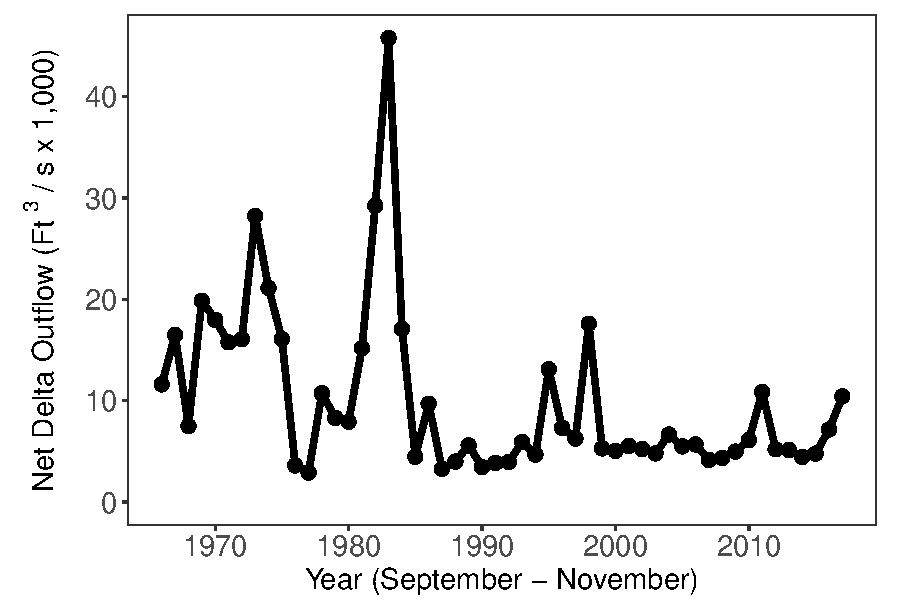
\includegraphics[width=\maxwidth]{figures/flow_fig_1-1} 

}



  \end{Cell}
\end{Row}

\vspace{-0cm}

\begin{Row}
   \begin{Cell}{1}
			\hspace{42pt}
			\begin{minipage}{195pt}
				\fcolorbox{black}[HTML]{27408B}{\parbox[c][12pt]{\textwidth}{
					\begin{center}
						{\LARGE \textcolor{white}{San Pablo Bay}}
					\end{center}
				}}
			\end{minipage}% This must go next to `\end{minipage}`
			\hspace{62pt}
			\begin{minipage}{195pt}
				\fcolorbox{black}[HTML]{27408B}{\parbox[c][12pt]{\textwidth}{
					\begin{center}
						{\LARGE \textcolor{white}{Suisun Bay}}
					\end{center}
				}}
			\end{minipage}% This must go next to `\end{minipage}`			
			\hspace{62pt}
			\begin{minipage}{195pt}
				\fcolorbox{black}[HTML]{27408B}{\parbox[c][12pt]{\textwidth}{
					\begin{center}
						{\LARGE \textcolor{white}{Delta}}
					\end{center}
				}}
			\end{minipage}
   \end{Cell}
\end{Row}

\vspace{-0.2cm}

\begin{Row}
    \begin{Cell}{1}
      %\includegraphics[align=m,width=1.0\textwidth]{figures/main_fig.PNG}


{\centering 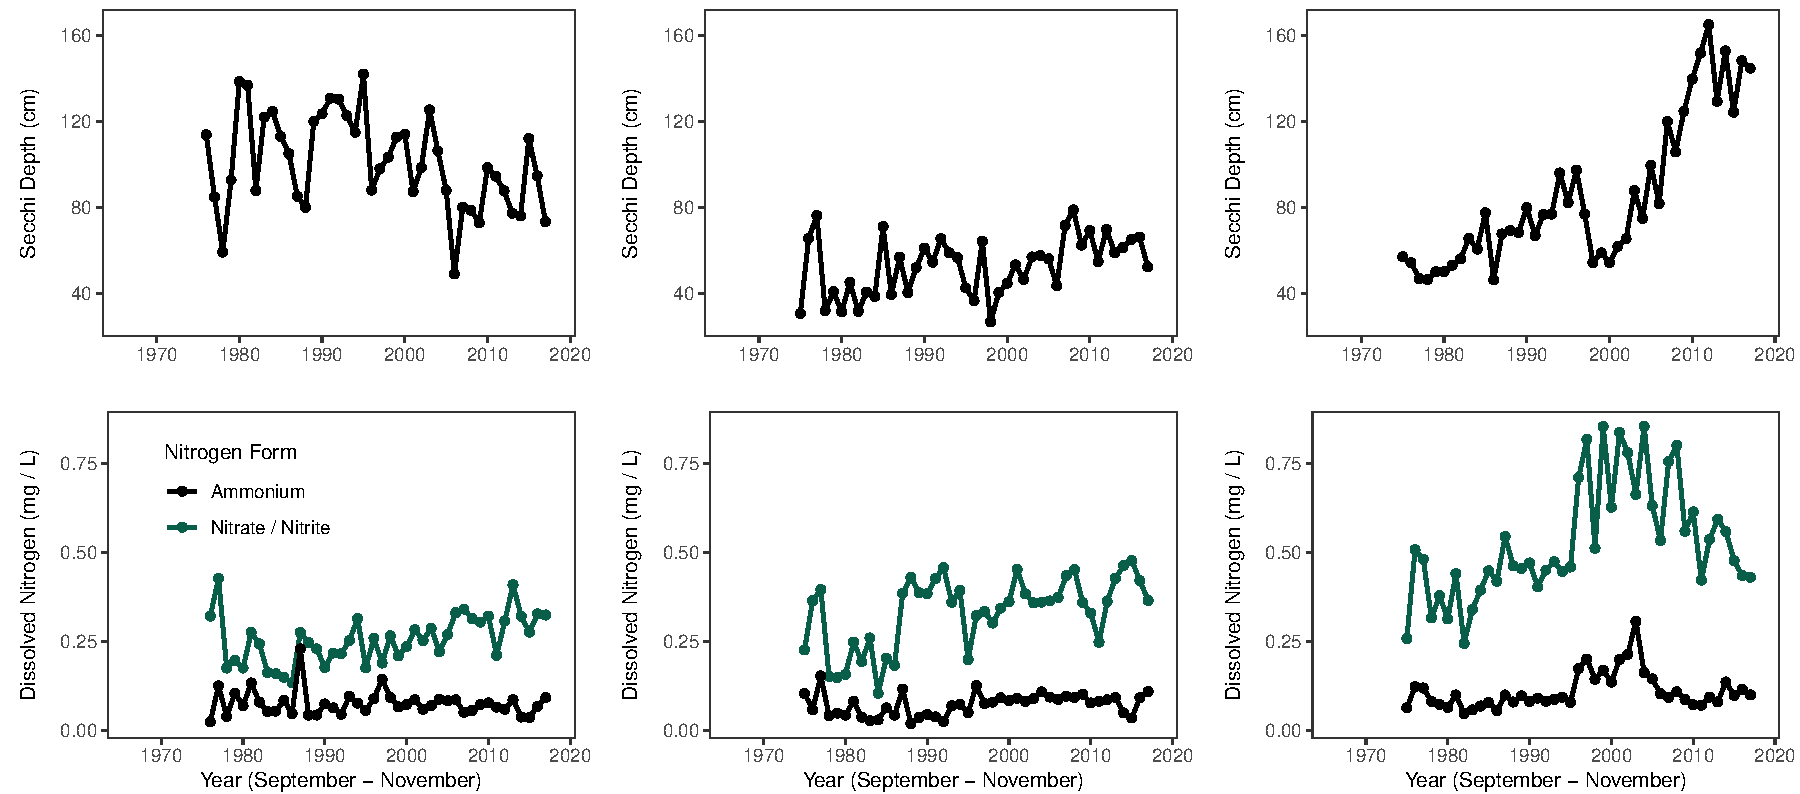
\includegraphics[width=\maxwidth]{figures/water_quality_main_fig-1} 

}



		\end{Cell}
\end{Row}

\vspace{0.2cm}

\begin{Row}
    \begin{Cell}{14}
      \textbf{\underline{FOR MORE INFORMATION}}: The 
			\href{https://water.ca.gov/Programs/Environmental-Services/Compliance-Monitoring-And-Assessment/Dayflow-Data}{California Estuary Portal} 
			provides access to raw and summarized water quality data for the 
			Sacramento-San Joaquin Delta. The 
			\href{https://water.ca.gov/Programs/Environmental-Services/Compliance-Monitoring-And-Assessment/Dayflow-Data}{California Department of Water Resources} 
			provides information and data on outflow. The IEP website provides the 
			\href{https://water.ca.gov/-/media/DWR-Website/Web-Pages/Programs/Environmental-Services/Interagency-Ecological-Program/Files/Interagency-Ecological-Program-Status-and-Trends-Fall-2017.pdf}{metadata} 
			for production of this report.
    \end{Cell}
    \begin{Cell}{2}

    \end{Cell}
\end{Row}


\newpage



%%%% Plankton:
\begin{Row}
  \begin{Cell}{1}
    \begin{center}
      
\includegraphics[align=m,height=2cm]{figures/IEP_logo.PNG}
    \end{center}
  \end{Cell}
  \begin{Cell}{6}
    \begin{center}
      \vspace{-0.8cm}		% Manually deal with the extra whitespace
      \doublespacing
      {\Large Interagency Ecological Program Status \& Trends } \\
      \vspace{0.2cm}
      {\Huge 2017 Fall Season Report} \\
      {\Large \emph{Plankton: 1975 -- 2017}}
    \end{center}
  \end{Cell}
  \begin{Cell}{1}
    \begin{center}
      
\includegraphics[align=m,height=1.9cm]{figures/fall_logo.PNG}
    \end{center}
  \end{Cell}
  \begin{Cell}{4}
  \end{Cell}
\end{Row}

\begin{Row}
  \begin{Cell}{2}
    \setlength{\fboxrule}{1.7pt}
    \fcolorbox{black}[HTML]{FFEEBA}{\parbox{\textwidth}{
			\begin{itemize}[leftmargin=*]
				{\large 
					\item Plankton densities and composition have shown large shifts since 
					surveys began in 1975.
					\item The most dramatic shift occurred after invasion of the overbite clam 
					in 1986. Filter feeding by these clams caused a substantial decline in 
					chlorophyll-a, a proxy for phytoplankton productivity.
					\item Zooplankton represent an import food source for many fishes, and like 
					phytoplankton, declined after arrival of the overbite clam. Mysids, calanoid 
					copepods, and cladocerans are large-bodied zooplankton and generally offer a 
					more nutritious food source compared to the relatively smaller cyclopoid 
					copepods.
				}
			\end{itemize}
    }}
  \end{Cell}
  \begin{Cell}{1}
    \vspace{-3.5cm}


{\centering 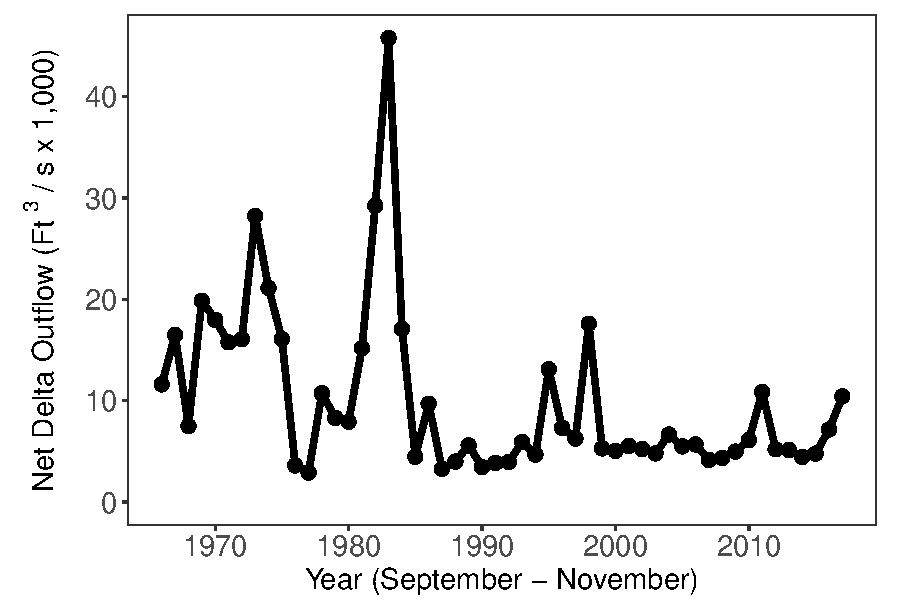
\includegraphics[width=\maxwidth]{figures/flow_fig_2-1} 

}



  \end{Cell}
\end{Row}

\vspace{-0cm}

\begin{Row}
   \begin{Cell}{1}
			\hspace{42pt}
			\begin{minipage}{195pt}
				\fcolorbox{black}[HTML]{27408B}{\parbox[c][12pt]{\textwidth}{
					\begin{center}
						{\LARGE \textcolor{white}{San Pablo Bay}}
					\end{center}
				}}
			\end{minipage}% This must go next to `\end{minipage}`
			\hspace{62pt}
			\begin{minipage}{195pt}
				\fcolorbox{black}[HTML]{27408B}{\parbox[c][12pt]{\textwidth}{
					\begin{center}
						{\LARGE \textcolor{white}{Suisun Bay}}
					\end{center}
				}}
			\end{minipage}% This must go next to `\end{minipage}`			
			\hspace{62pt}
			\begin{minipage}{195pt}
				\fcolorbox{black}[HTML]{27408B}{\parbox[c][12pt]{\textwidth}{
					\begin{center}
						{\LARGE \textcolor{white}{Delta}}
					\end{center}
				}}
			\end{minipage}
   \end{Cell}
\end{Row}

\vspace{-0.2cm}

\begin{Row}
    \begin{Cell}{1}


{\centering 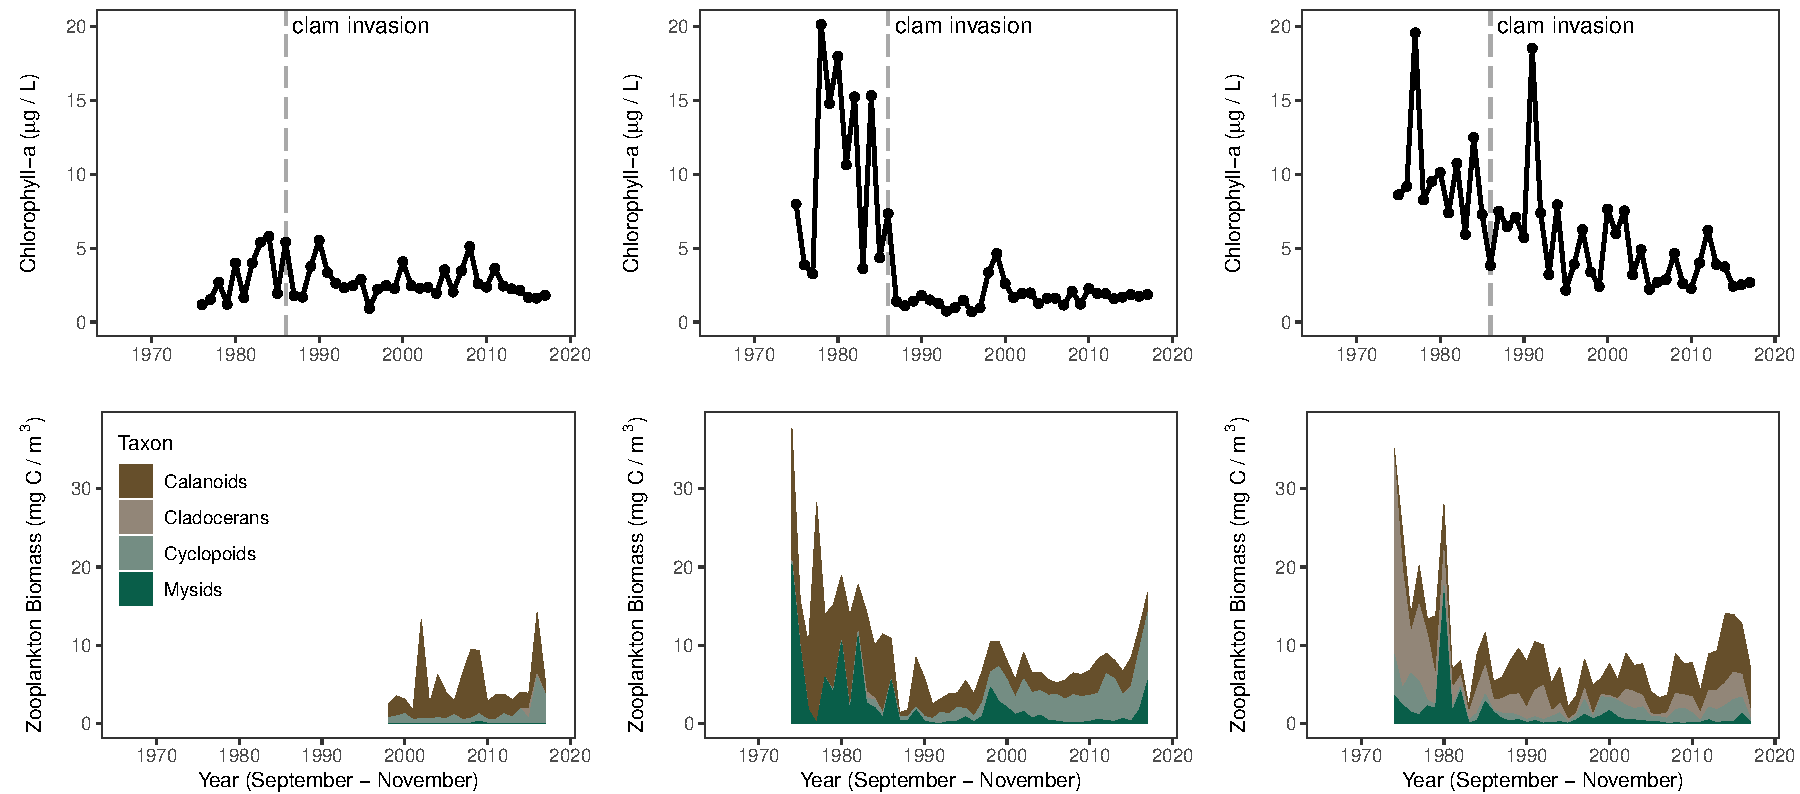
\includegraphics[width=\maxwidth]{figures/plankton_main_fig-1} 

}



		\end{Cell}
\end{Row}

\vspace{0.2cm}

\begin{Row}
    \begin{Cell}{14}
      \textbf{\underline{FOR MORE INFORMATION}}: Recent articles in the IEP Newsletter 
			summarize status and trends of 
			\href{https://water.ca.gov/-/media/DWR-Website/Web-Pages/Programs/Environmental-Services/Interagency-Ecological-Program/Files/Newsletters/IEP-Newsletter-Vol29-Issue2---2016.pdf}{phyotoplankton} 
			and \href{https://water.ca.gov/-/media/DWR-Website/Web-Pages/Programs/Environmental-Services/Interagency-Ecological-Program/Files/Newsletters/IEP-Newsletter-Vol30-Issue1---2017.pdf}{zooplankton},
			including a \href{https://water.ca.gov/-/media/DWR-Website/Web-Pages/Programs/Environmental-Services/Interagency-Ecological-Program/Files/Newsletters/IEP-Newsletter-Vol30-Issue2---2017.pdf}{recent phyotoplankton bloom} in Spring 2016. The IEP website 
			provides the \href{https://water.ca.gov/-/media/DWR-Website/Web-Pages/Programs/Environmental-Services/Interagency-Ecological-Program/Files/Interagency-Ecological-Program-Status-and-Trends-Fall-2017.pdf}{metadata} for production of this report.
    \end{Cell}
    \begin{Cell}{2}

    \end{Cell}
\end{Row}



\newpage



%%%% Fish 1:
\begin{Row}
  \begin{Cell}{1}
    \begin{center}
      
\includegraphics[align=m,height=2cm]{figures/IEP_logo.PNG}
    \end{center}
  \end{Cell}
  \begin{Cell}{6}
    \begin{center}
      \vspace{-0.8cm}		% Manually deal with the extra whitespace
      \doublespacing
      {\Large Interagency Ecological Program Status \& Trends } \\
      \vspace{0.2cm}
      {\Huge 2017 Fall Season Report} \\
      {\Large \emph{Fishes: 1967 -- 2017}}
    \end{center}
  \end{Cell}
  \begin{Cell}{1}
    \begin{center}
      
\includegraphics[align=m,height=1.9cm]{figures/fall_logo.PNG}
    \end{center}
  \end{Cell}
  \begin{Cell}{4}
  \end{Cell}
\end{Row}

\begin{Row}
  \begin{Cell}{2}
    \setlength{\fboxrule}{1.7pt}
    \fcolorbox{black}[HTML]{FFEEBA}{\parbox{\textwidth}{
			\begin{itemize}[leftmargin=*]
				{\large 
					\item The Fall Midwater Trawl began in 1967 and surveys the pelagic, or 
					open water, fish community. Indices for many pelagic fishes are at record lows, 
					including Delta and Longfin Smelt, which are protected by California and/or 
					federal Endangered Species Acts.
					\item White sturgeon is a species of concern and a popular target of 
					recreational fishing. Catch per unit effort is based on trammel net surveys.
					\item Fall Run Chinook Salmon, an important species for both the commercial 
					and recreational fishery, is also a species of concern. Population dynamics 
					are driven by hatchery production and a suite of environmental variables. 
					Total counts of both in-river and hatchery returns are shown here.
				}
			\end{itemize}
    }}
  \end{Cell}
  \begin{Cell}{1}
    \vspace{-4.0cm}


{\centering 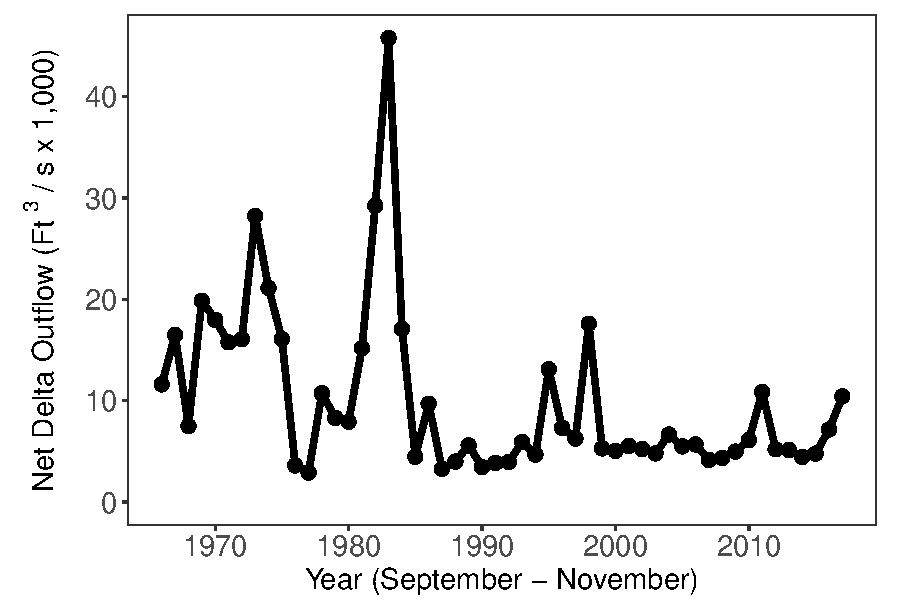
\includegraphics[width=\maxwidth]{figures/flow_fig_3-1} 

}



  \end{Cell}
\end{Row}

\vspace{0cm}

\begin{Row}
   \begin{Cell}{1}
			\hspace{35pt}
			\begin{minipage}{466pt}
				\fcolorbox{black}[HTML]{27408B}{\parbox[c][12pt]{\textwidth}{
					\begin{center}
						{\LARGE \textcolor{white}{Fall Midwater Trawl}}
					\end{center}
				}}
			\end{minipage}% This must go next to `\end{minipage}`
			\hspace{52pt}
			\begin{minipage}{205pt}
				\fcolorbox{black}[HTML]{27408B}{\parbox[c][12pt]{\textwidth}{
					\begin{center}
						{\LARGE \textcolor{white}{Other Surveys}}
					\end{center}
				}}
			\end{minipage}
   \end{Cell}
\end{Row}

\vspace{-0.2cm}

\begin{Row}
    \begin{Cell}{1}


{\centering 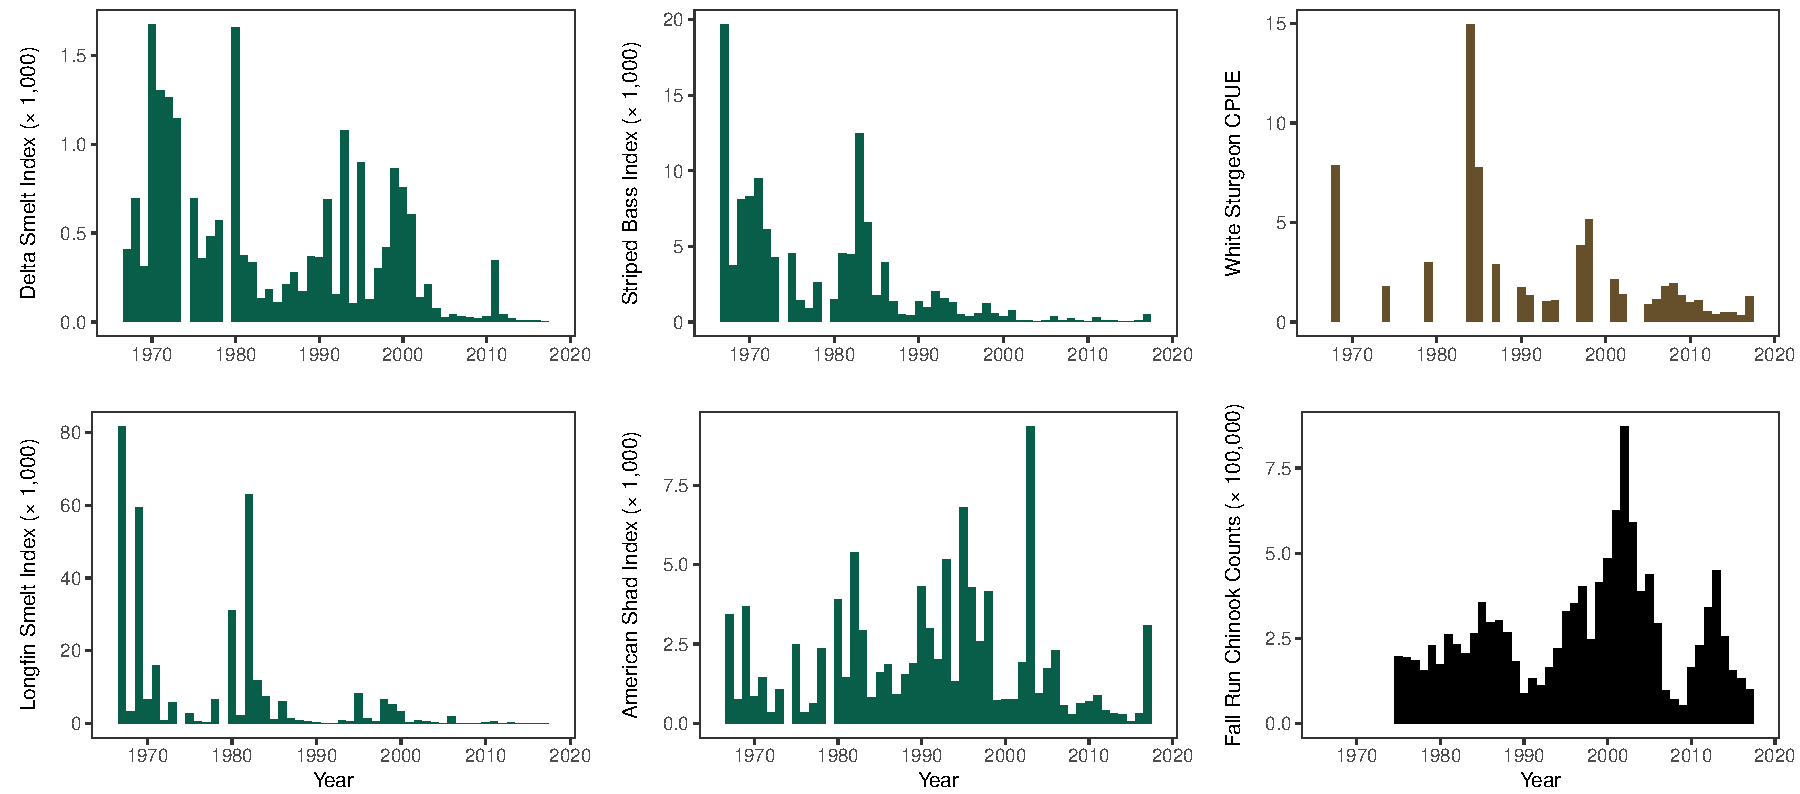
\includegraphics[width=\maxwidth]{figures/fish1_main_fig-1} 

}



		\end{Cell}
\end{Row}

\vspace{0.2cm}

\begin{Row}
    \begin{Cell}{14}
      \textbf{\underline{FOR MORE INFORMATION}}: Recent articles in the IEP Newsletter 
			summarize trends and abundance index calculations for 
			\href{https://water.ca.gov/-/media/DWR-Website/Web-Pages/Programs/Environmental-Services/Interagency-Ecological-Program/Files/Newsletters/IEP-Newsletter-Vol30-Issue2---2017.pdf}{pelagic fishes}. 
			The IEP website provides the 
			\href{https://water.ca.gov/-/media/DWR-Website/Web-Pages/Programs/Environmental-Services/Interagency-Ecological-Program/Files/Interagency-Ecological-Program-Status-and-Trends-Fall-2017.pdf}{metadata} 
			for production of this report.
    \end{Cell}
    \begin{Cell}{2}

    \end{Cell}
\end{Row}



\newpage



%%%% Fish 2:
\begin{Row}
  \begin{Cell}{1}
    \begin{center}
      
\includegraphics[align=m,height=2cm]{figures/IEP_logo.PNG}
    \end{center}
  \end{Cell}
  \begin{Cell}{6}
    \begin{center}
      \vspace{-0.8cm}		% Manually deal with the extra whitespace
      \doublespacing
      {\Large Interagency Ecological Program Status \& Trends } \\
      \vspace{0.2cm}
      {\Huge 2017 Fall Season Report} \\
      {\Large \emph{Fishes: 2002 -- 2017}}
    \end{center}
  \end{Cell}
  \begin{Cell}{1}
    \begin{center}
      
\includegraphics[align=m,height=1.9cm]{figures/fall_logo.PNG}
    \end{center}
  \end{Cell}
  \begin{Cell}{4}
  \end{Cell}
\end{Row}

\begin{Row}
  \begin{Cell}{2}
    \setlength{\fboxrule}{1.7pt}
    \fcolorbox{black}[HTML]{FFEEBA}{\parbox{\textwidth}{
			\begin{itemize}[leftmargin=*]
				{\large 
					\item Many pelagic fishes declined sharply around 2001 in what is known as 
					the Pelagic Organism Decline. Some species have continued to decline over the 
					last 15 years.
					\item For Delta Smelt, 2017 marked the lowest recorded index in over 50 
					years (Index = 2).
					\item Some fish species increased in 2017 relative to recent years. The 
					Striped Bass 2017 index was the highest since 2001. The 2017 Longfin Smelt 
					index was the highest since 2013. American Shad saw its highest index since 
					2003, and White Sturgeon CPUE was the highest since 2009.
					\item In 2017, Fall Run Chinook Salmon declined for the fourth year in a 
					row (counts = 101,222).
				}
			\end{itemize}
    }}
  \end{Cell}
  \begin{Cell}{1}
    \vspace{-4.0cm}


{\centering 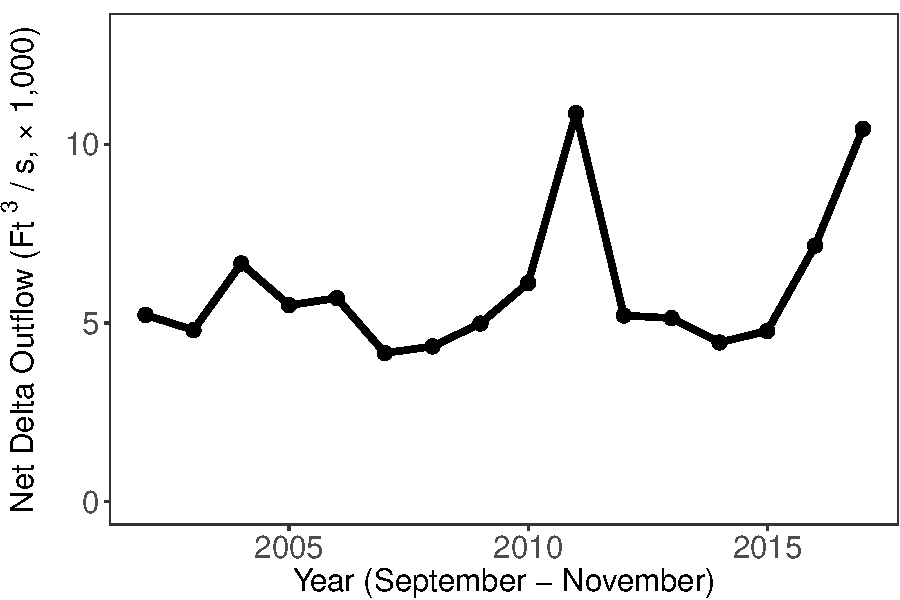
\includegraphics[width=\maxwidth]{figures/flow_fig_4-1} 

}



  \end{Cell}
\end{Row}

\vspace{0cm}

\begin{Row}
   \begin{Cell}{1}
			\hspace{35pt}
			\begin{minipage}{466pt}
				\fcolorbox{black}[HTML]{27408B}{\parbox[c][12pt]{\textwidth}{
					\begin{center}
						{\LARGE \textcolor{white}{Fall Midwater Trawl}}
					\end{center}
				}}
			\end{minipage}% This must go next to `\end{minipage}`
			\hspace{52pt}
			\begin{minipage}{205pt}
				\fcolorbox{black}[HTML]{27408B}{\parbox[c][12pt]{\textwidth}{
					\begin{center}
						{\LARGE \textcolor{white}{Other Surveys}}
					\end{center}
				}}
			\end{minipage}
   \end{Cell}
\end{Row}

\vspace{-0.2cm}

\begin{Row}
    \begin{Cell}{1}


{\centering 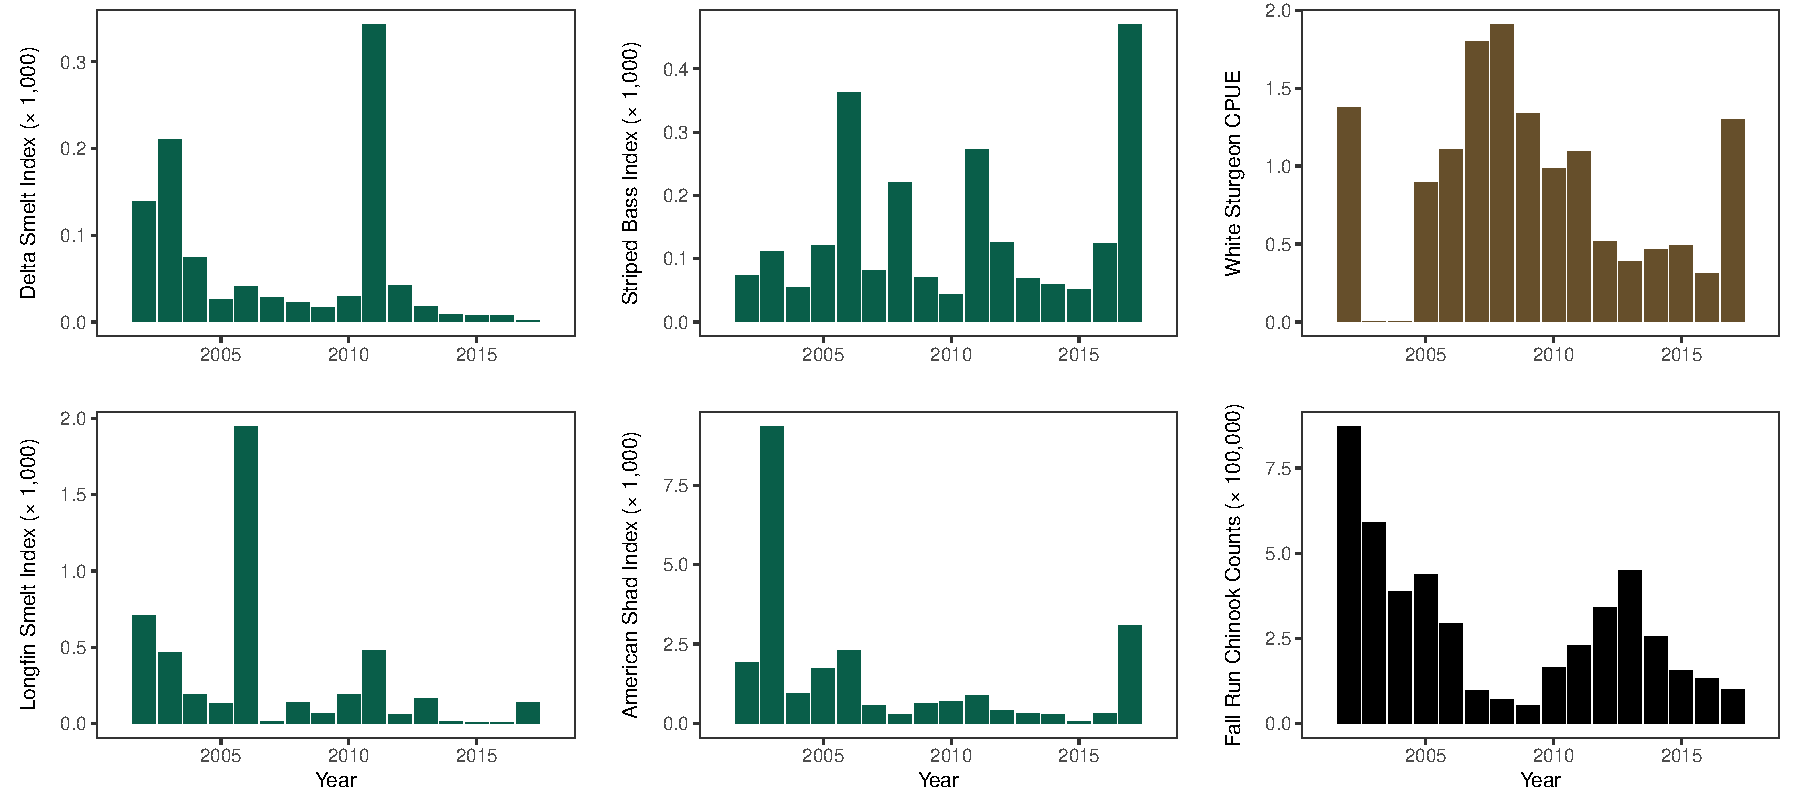
\includegraphics[width=\maxwidth]{figures/fish2_main_fig-1} 

}



		\end{Cell}
\end{Row}

\vspace{0.2cm}

\begin{Row}
    \begin{Cell}{14}
      \textbf{\underline{FOR MORE INFORMATION}}: The  
			\href{https://www.wildlife.ca.gov/Regions/3}{California Department of Fish and Wildlife} provides information and 
			data for the Fall Midwater Trawl and Sturgeon study. 
			\href{http://www.calfish.org/ProgramsData/Species/CDFWAnadromousResourceAssessment.aspx}{CalFish} provides Chinook Salmon data via the GrandTab database. 
			The IEP website provides the 
			\href{https://water.ca.gov/-/media/DWR-Website/Web-Pages/Programs/Environmental-Services/Interagency-Ecological-Program/Files/Interagency-Ecological-Program-Status-and-Trends-Fall-2017.pdf}{metadata} 
			for production of this report.
    \end{Cell}
    \begin{Cell}{2}

    \end{Cell}
\end{Row}


\end{document}
